
\subsection{Introducción}
Se realizaron simulaciones en LTSpice del circuito propuesto, así también se comprobó que los resultados teóricos concuerdan con las simulaciones, ademas se tuvo especial cuidado a la hora de evaluar que transistores y resistores usar en las etapas tal que no haya problemas de potencia, aqui se muestran las tensiones y potenicas relevantes del circuito en cuanto a la elección crítica de componentes.\\
Comenzando por los emisores comunes la potencia se encuentra cerca del máximo y la tensión Vce en un rango seguro.

\begin{figure}[H]
	\centering
	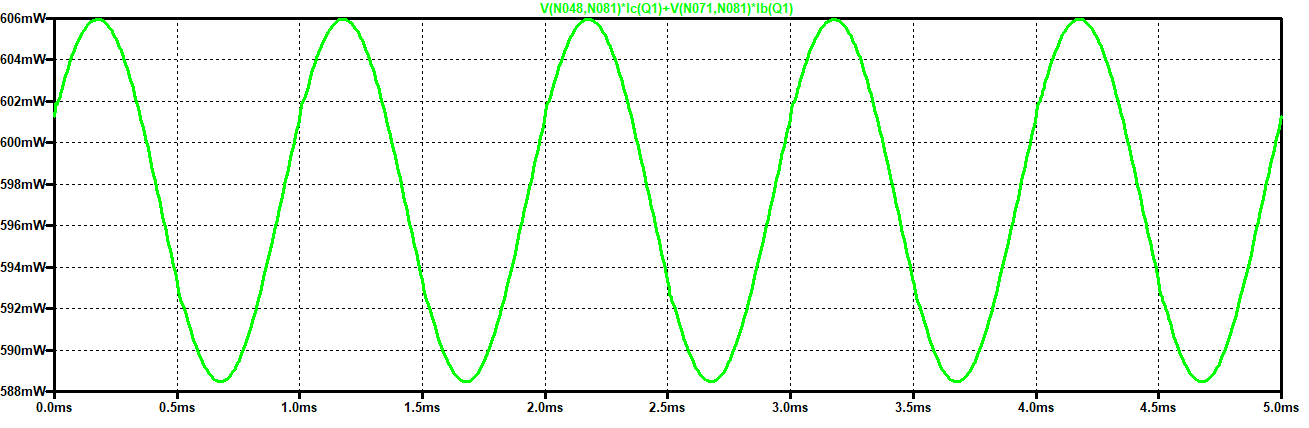
\includegraphics[width=0.8\textwidth]{ImagenesSimulaciones/PEC1.png}
		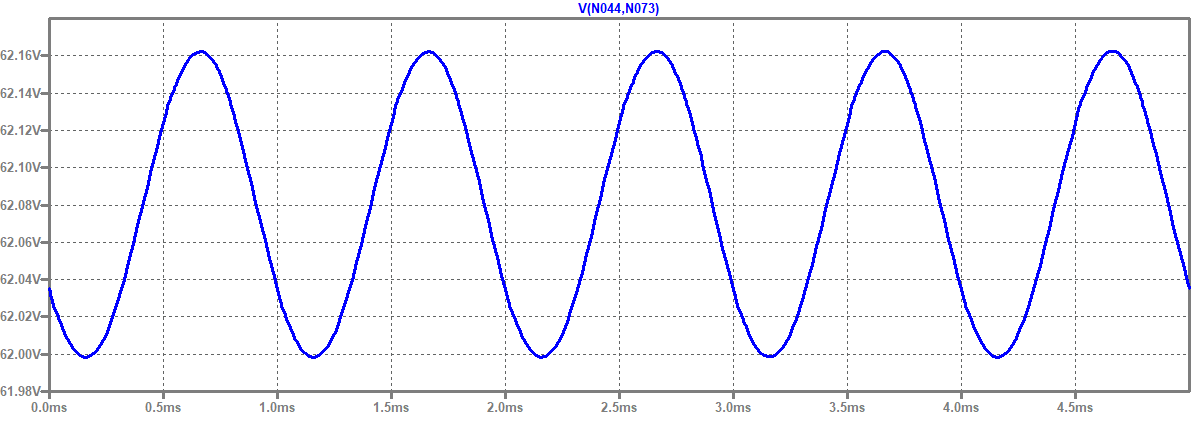
\includegraphics[width=0.8\textwidth]{ImagenesSimulaciones/VEC1.png}
	\caption{Potencia y tensión sobre un emisor común sin carga activa.}
	\label{fig:pec1}
\end{figure}También se cuenta con que la potencia disipada por las resistencias de colector son cercanas al medio watt, por lo que las resistencias a utilizar son de medio watt.\\
Luego el úlitmo emisor común, el cual tiene la mayor ganancia de todos, es razonable esperar que disipe mas potencia y en efecto así es, por eso la necesidad de utilizar un transistor de mayor potencia para este ademas de que este manejara la máxima variación de tensión.

\begin{figure}[H]
	\centering
	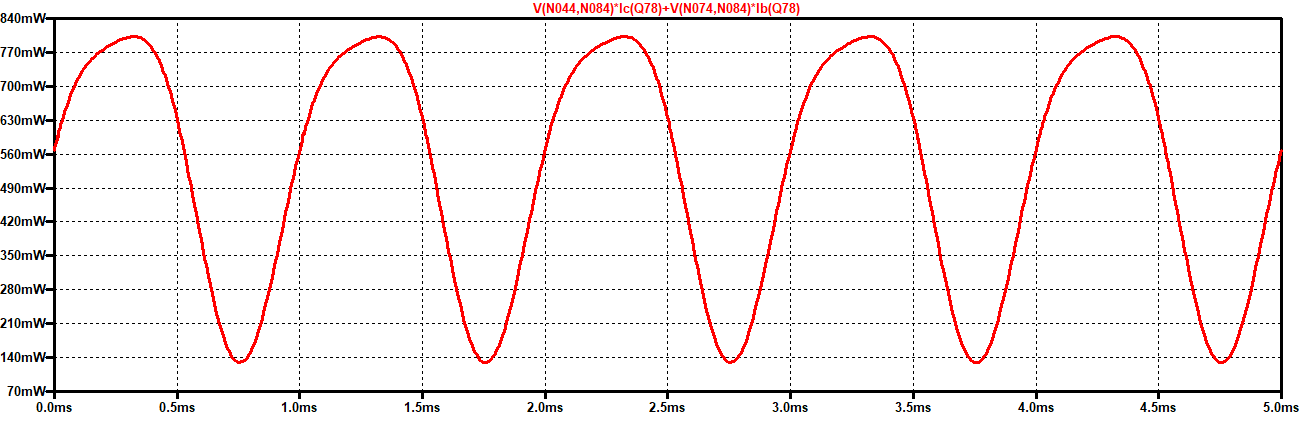
\includegraphics[width=0.8\textwidth]{ImagenesSimulaciones/PECF.png}
		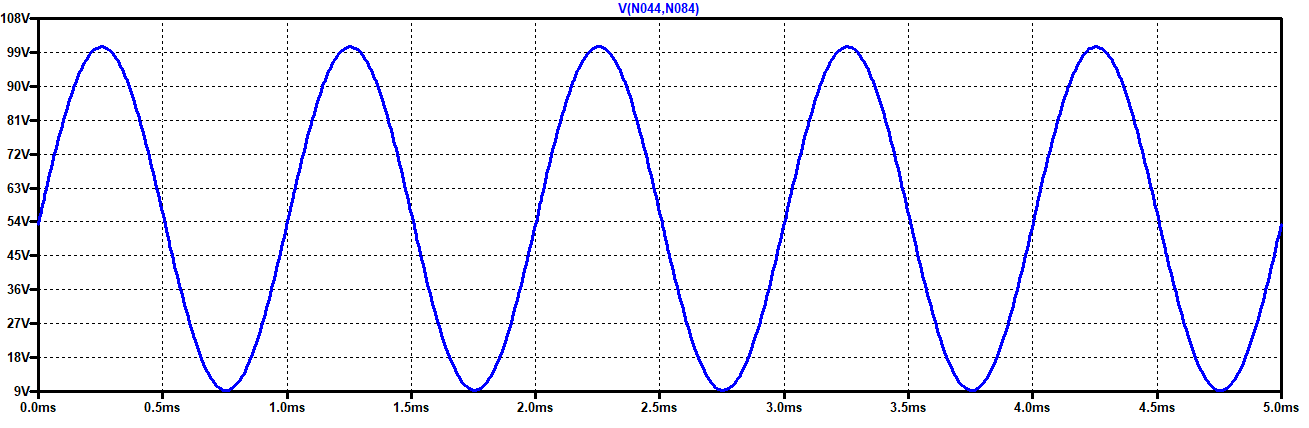
\includegraphics[width=0.8\textwidth]{ImagenesSimulaciones/VECF.png}
	\caption{Potencia y tensión sobre un emisor común con carga activa.}
	\label{fig:pecf}
\end{figure}
%% potencai fuente de corriente de la carga activa
En cuanto a la carga activa, dado que se encuentra en el colector del transistor va a  sufrir también una gran variación de tensión por lo que se necesita un transistor que pueda manejar dicha tensión.
\begin{figure}[H]
	\centering
	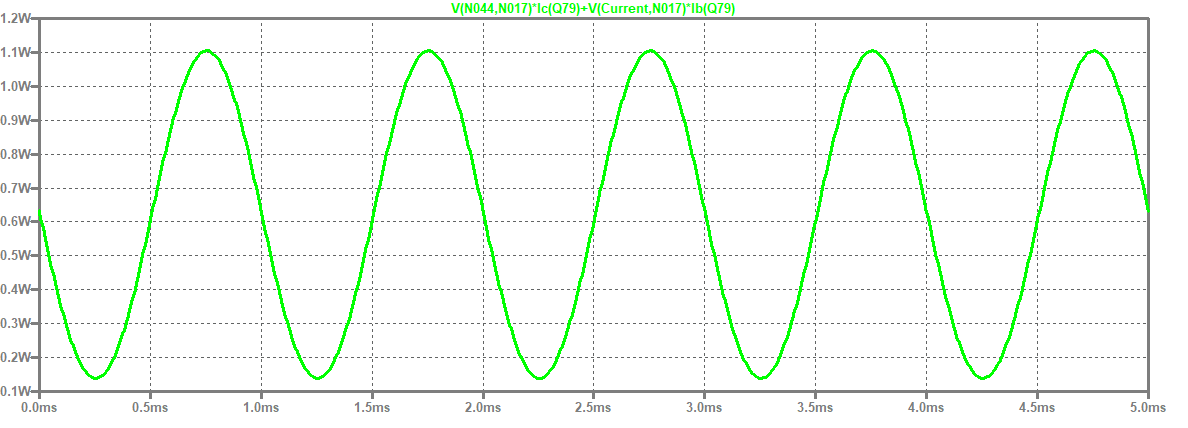
\includegraphics[width=0.8\textwidth]{ImagenesSimulaciones/PCSEC.png}
		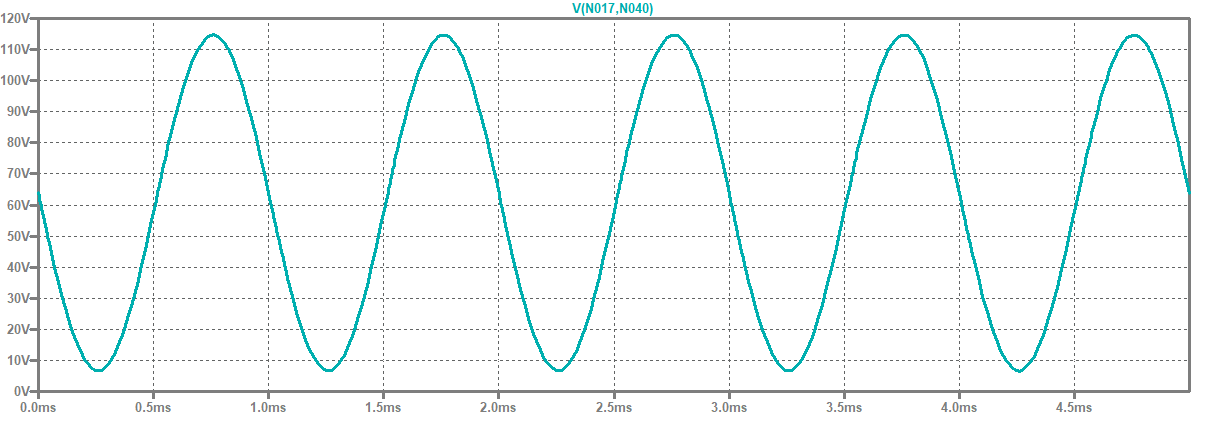
\includegraphics[width=0.8\textwidth]{ImagenesSimulaciones/VCSEC.png}
	\caption{Potencia y tensión sobre la carga activa.}
	\label{fig:pcsecf}
\end{figure}

%% potencia de la fuente de corriente del multiplicador de vbe
Continuando por la potencia y tensión correspondiente a la fuente de corriente de la etapa de salida.
\begin{figure}[H]
	\centering
	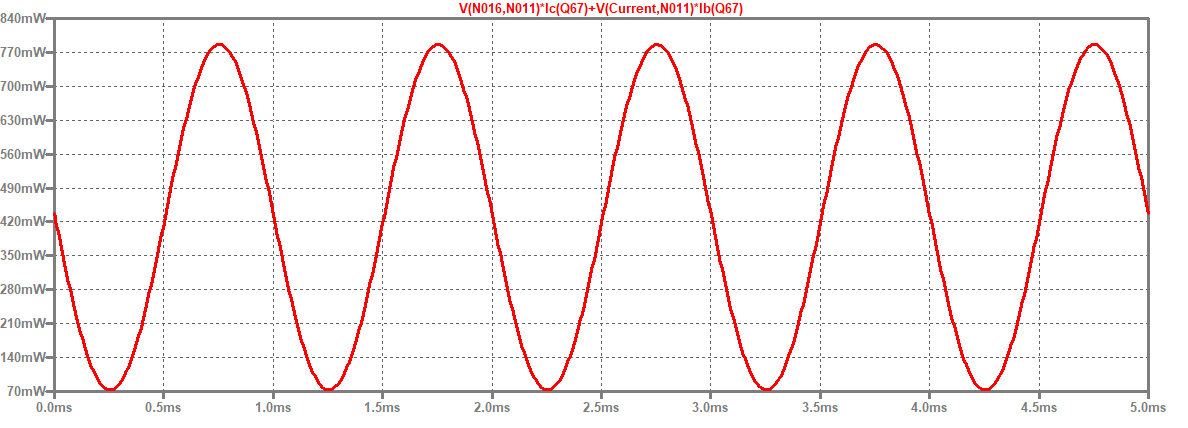
\includegraphics[width=0.8\textwidth]{ImagenesSimulaciones/PCSVBE.png}
		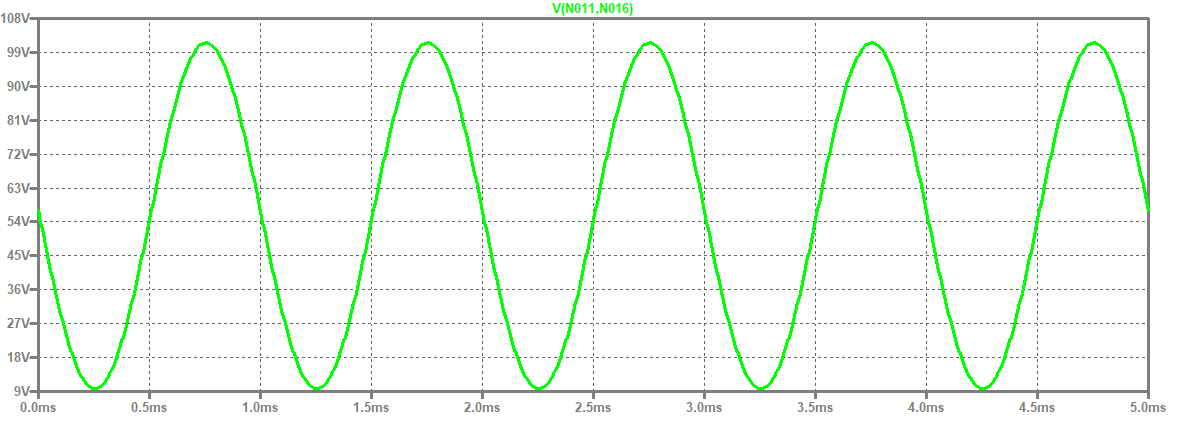
\includegraphics[width=0.8\textwidth]{ImagenesSimulaciones/VCSVBE.png}
	\caption{Potencia y tensión de la fuente de corriente de la salida.}
	\label{fig:pcsvbe}
\end{figure}
%%potencia en el primer transistor de salida
Considerando la potencia de la etapa de salida consideraremos la potencia de las 3 fases, correspondiendo a la primera, la de menor potencia:
\begin{figure}[H]
	\centering
	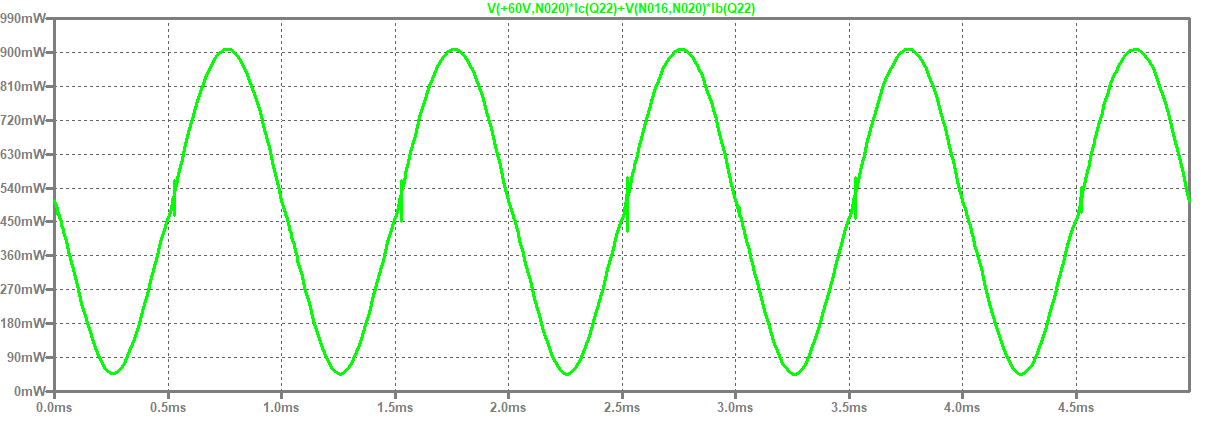
\includegraphics[width=0.8\textwidth]{ImagenesSimulaciones/PO1.png}
		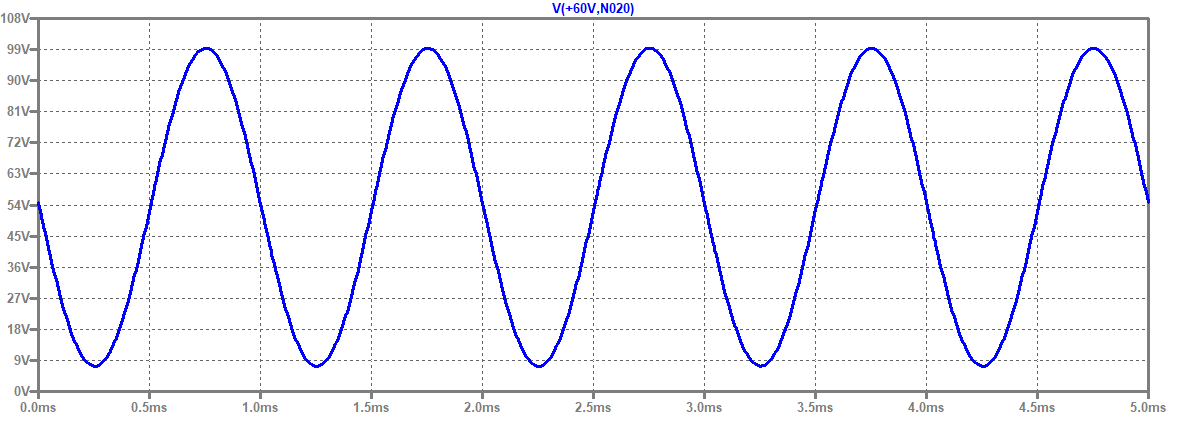
\includegraphics[width=0.8\textwidth]{ImagenesSimulaciones/VO1.png}
	\caption{Potencia y tensión del primer transistor de salida.}
	\label{fig:po1}
\end{figure}
Para el segundo, el cual corresponde a mediana potencia:
\begin{figure}[H]
	\centering
	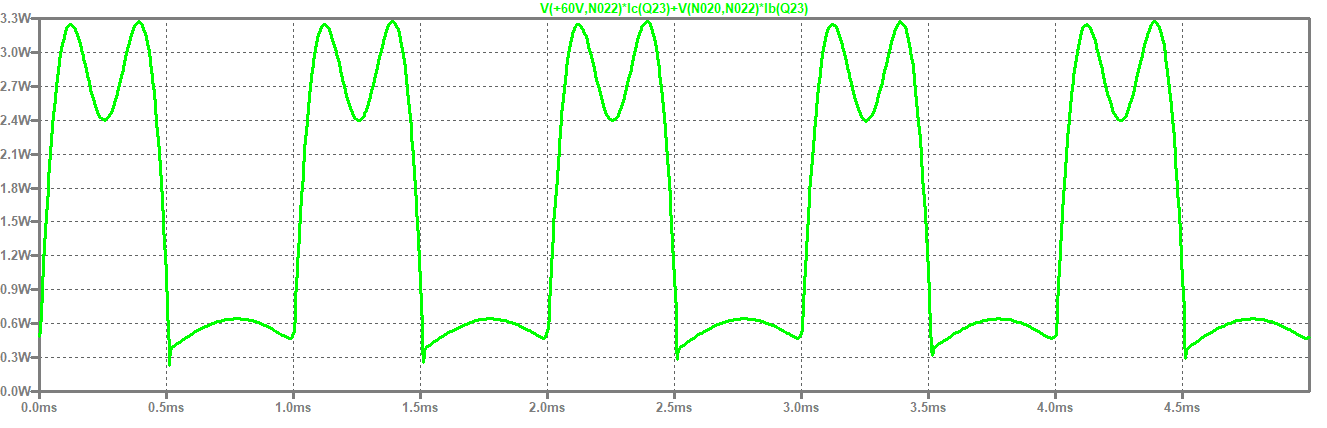
\includegraphics[width=0.8\textwidth]{ImagenesSimulaciones/PO2.png}
		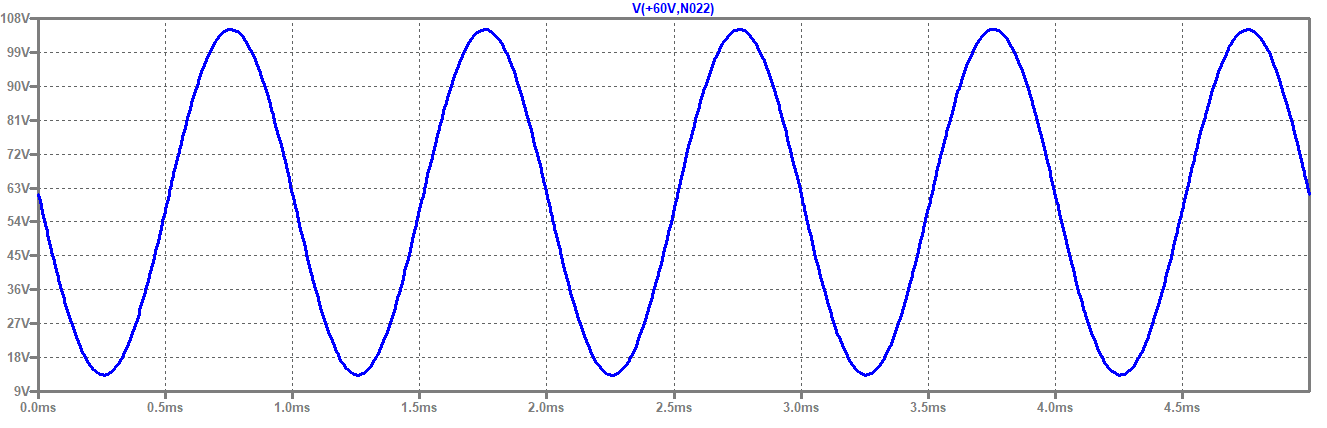
\includegraphics[width=0.8\textwidth]{ImagenesSimulaciones/VO2.png}
	\caption{Potencia y tensión del segundo transistor de salida.}
	\label{fig:po2}
\end{figure}
Finalmente para los últimos transistores, los cuales son los que trabajan con la mayor parte de la potencia de salida se obtuvo tanto la potencia como la tensión sobre ellos.
\begin{figure}[H]
	\centering
	\includegraphics[width=0.8\textwidth]{ImagenesSimulaciones/PO3.png}
		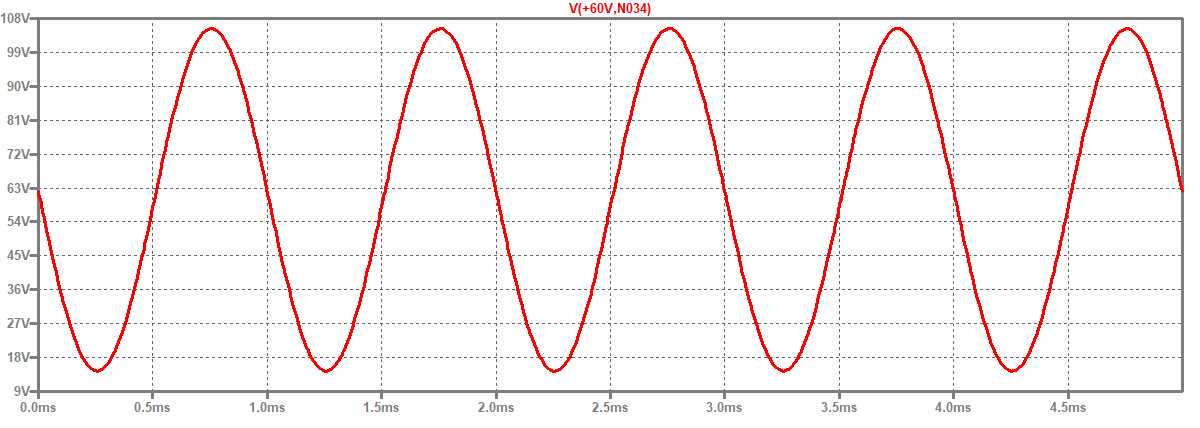
\includegraphics[width=0.8\textwidth]{ImagenesSimulaciones/VO3.png}
	\caption{Potencia y tensión de los transistores de salida.}
	\label{fig:po3}
\end{figure}
Adicional mente se puede observar que en el gráfico de potencias se dibujo también la potencia del transistor PNP de la rama inferior, para hacer evidente el nivel de simetría que se tiene.\\
Finalmente mostraremos la simulación de potencia sobre la carga.
\begin{figure}[H]
	\centering
	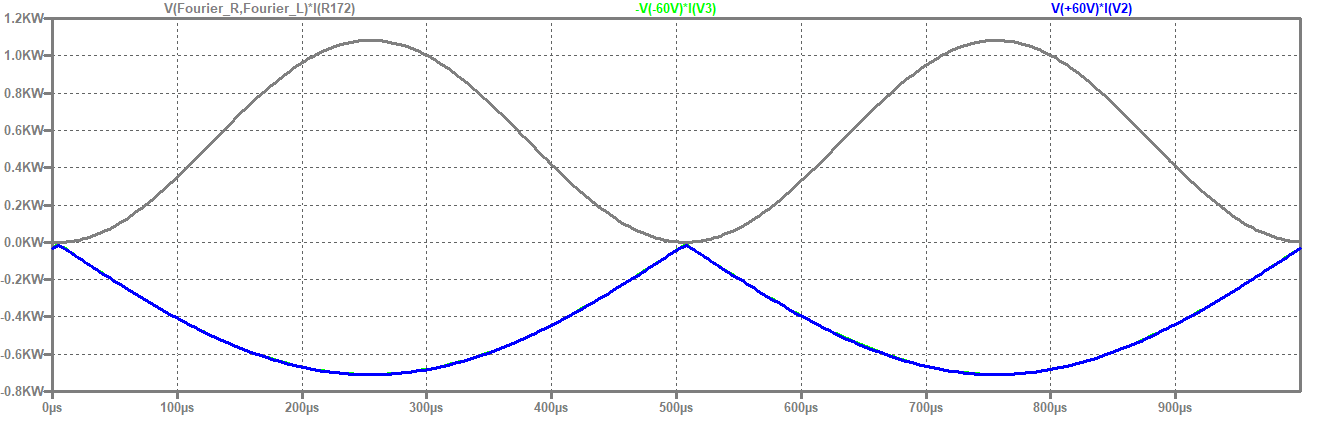
\includegraphics[width=0.8\textwidth]{ImagenesSimulaciones/PRL.png}
	\caption{Potencia sobre la carga.}
	\label{fig:porl}
\end{figure}
Aquí se pueden apreciar varias cosas, primeramente que con una tensión de entrada de 0.5$\hat{V}$ se obtiene la mayor potencia, la cual corresponde a $\approx 1078W$, también debe notarse que la potencia entregada por la fuente es $\approx 0W$ cuando la potencia sobre la carga también lo es.\\
Luego se obtuvo la salida del circuito teniendo a la entrada una señal senoidal de frecuencia 1KHz y de amplitud 0.25$\hat{V}$ y otra simulación con la misma entrada pero sumado también ruido blanco con distribución uniforme de amplitud $25m\hat{V}$.
\begin{figure}[H]
	\centering
	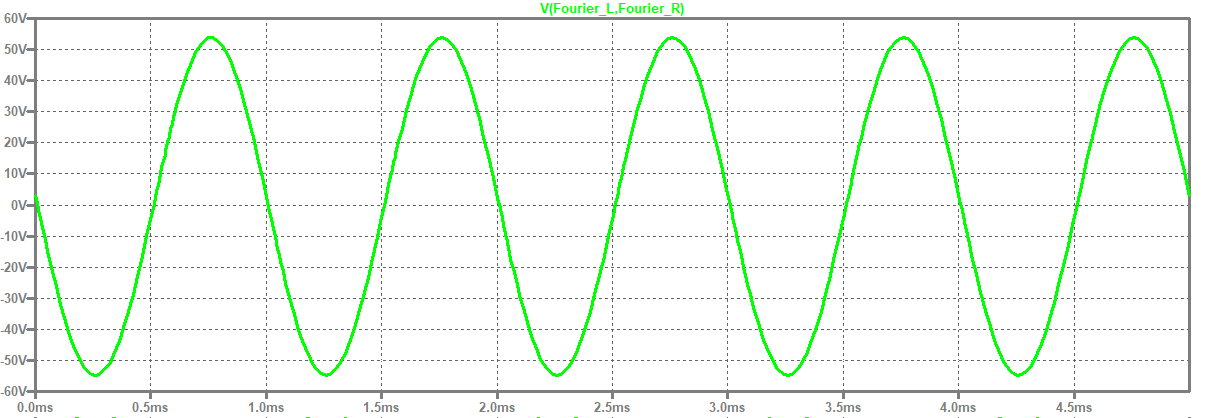
\includegraphics[width=0.8\textwidth]{ImagenesSimulaciones/VRL.png}
		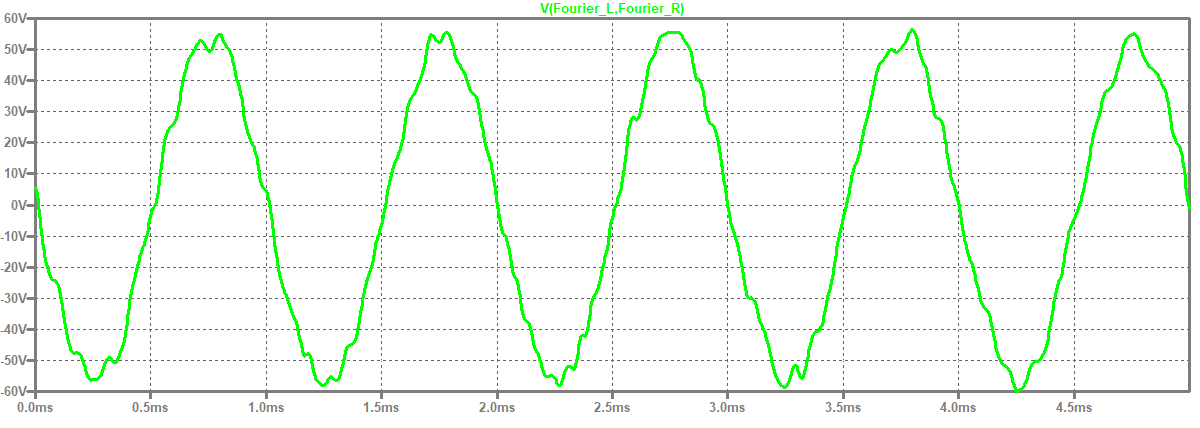
\includegraphics[width=0.8\textwidth]{ImagenesSimulaciones/VRLNoise.png}
	\caption{Tensión sobre la carga con y sin ruido.}
	\label{fig:VRLN}
\end{figure}
Finalmente se obtuvo el Bode del sistema como se observa a continuación:
\begin{figure}[H]
	\centering
	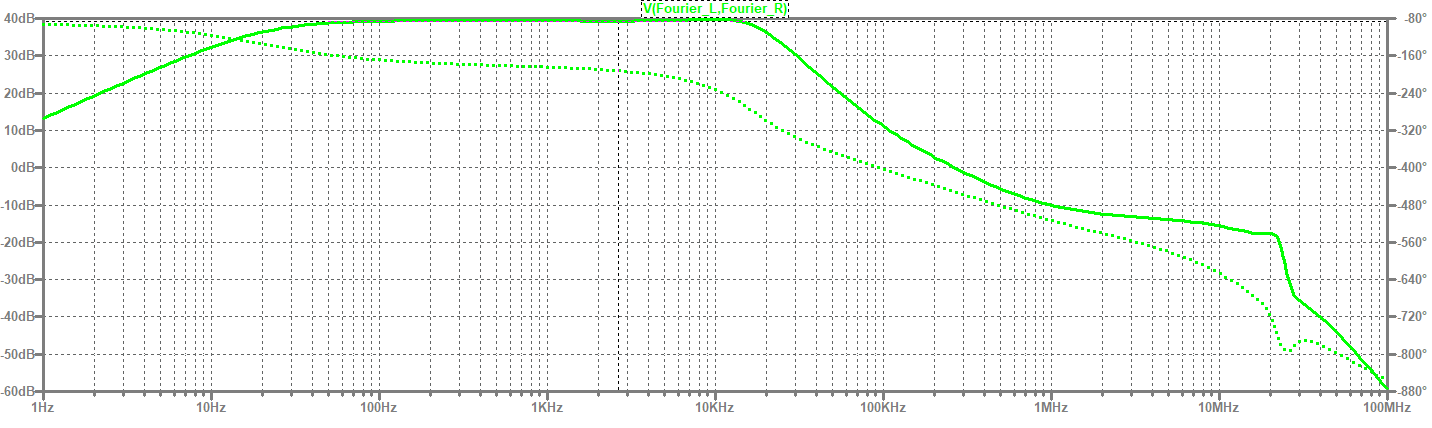
\includegraphics[width=0.9\textwidth]{ImagenesSimulaciones/BODE.png}
	\caption{Bode del sistema.}
	\label{fig:bode}
\end{figure}
Donde se puede apreciar una caida de 3dB respecto a la banda pasante tanto en 20Hz como en 20KHz.\\
También se simuló la impedancia tanto de entrada como de salida.
\begin{figure}[H]
	\centering
	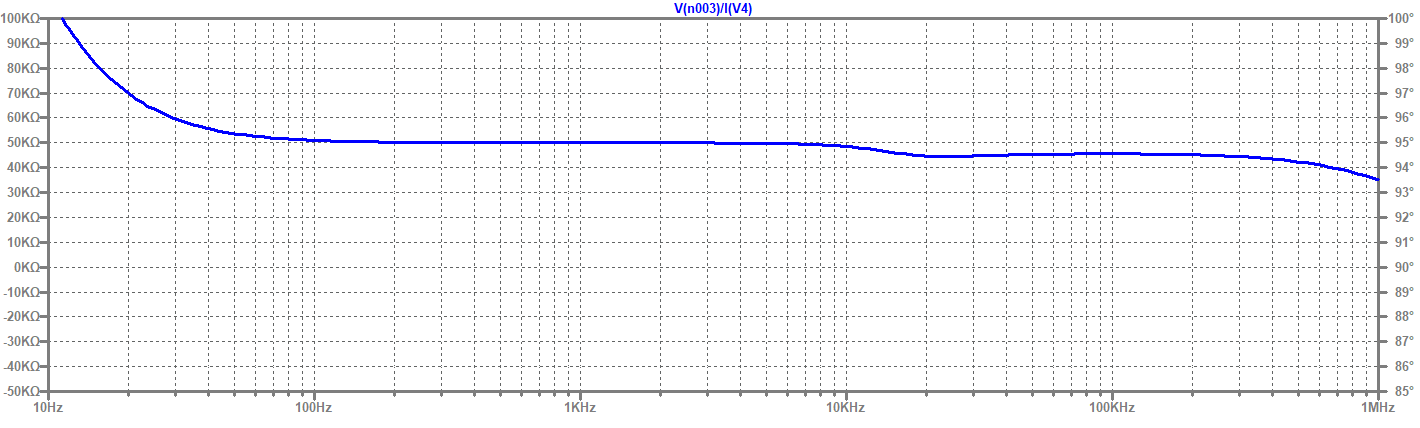
\includegraphics[width=0.9\textwidth]{ImagenesSimulaciones/Zin.png}
	\caption{Impedancia de entrada del sistema.}
	\label{fig:zin}
\end{figure}
Se puede notar que la impedancia de entrada en la banda audible es de 50K$\Omega$
\begin{figure}[H]
	\centering
	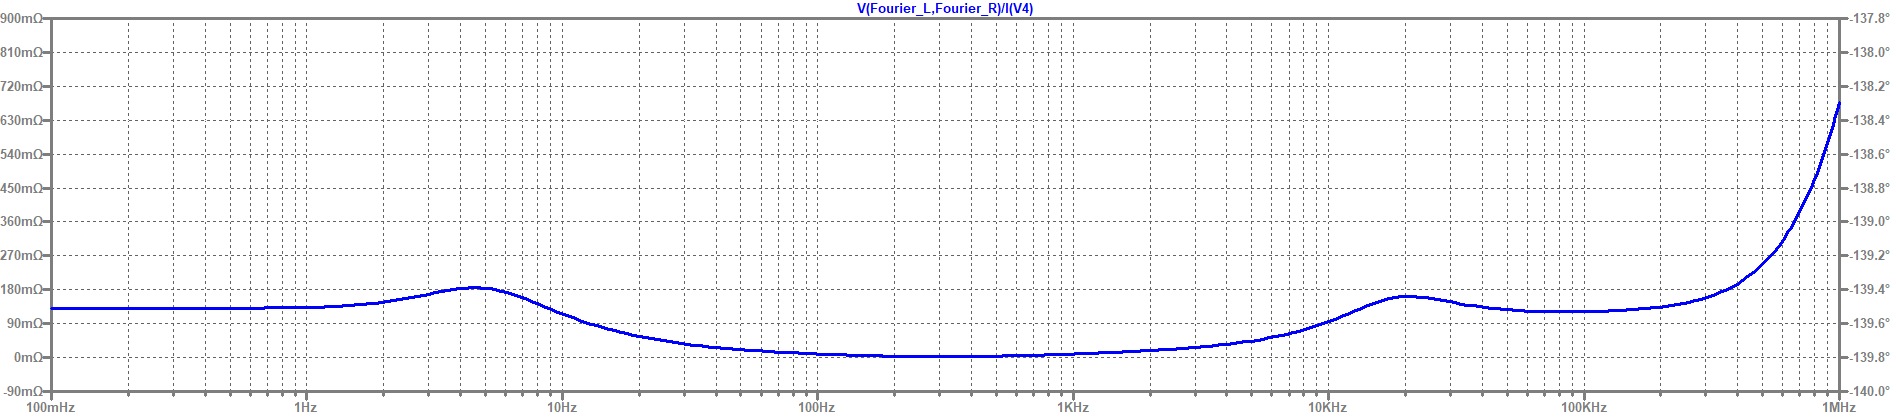
\includegraphics[width=0.9\textwidth]{ImagenesSimulaciones/Zout.png}
	\caption{Impedancia de salida del sistema.}
	\label{fig:zout}
\end{figure}
La impedancia de salida es un valor cercano del orden de las decenas de  m$\Omega$, idealmente sería de 8 $\Omega$ para que haya máxima transferencia de Potencia.
Como también se midió la THD en la simulación obteniendo un valor de 0.400742$\%$ cuando se disipa la máxima potencia.
%%Bode
